\section{Computational Results} \label{sec:Results}

The C-ITGO was implemented using Matlab, and the experiments were accomplished on a machine with the Intel i3-3110M CPU @2.40GHz processor with 4GB of RAM, running Windows 7. Also, we provide a free library for using C-ITGO for optimizing any user-defined function, being it constrained or not. The library uses by default the Matlab \textit{fmincon} solver for continuous problems and the OPTI toolbox (currently only readily available for Windows, but can be compiled for Linux and Mac as well) for mixed integer problems. Also, the user has the option to easily incorporate other local search algorithms, if desired.

%The source code for the reported results in this work can be found and downloaded for free at \cite{GIT}.

To evaluate the performance of the developed method to solve real-world problems, we use eight difficult constrained engineering optimization problems from the literature, whose objective functions and constraints are diverse (quadratic, cubic, polynomial and nonlinear) with many numbers and types of design variables (continuous, mixed and integer). 

In all tests, given the stochastic characteristic of C-ITGO, we run it 25 times, saving the Best and Worst feasible solutions, as well as the mean value (Mean) and standard deviation (SD) of the fitness after all runs. Given the great variability between the results found in the literature for most problems, we stop the execution of C-ITGO as soon as the best solution found in a run is considerably close to the optimum (the optimum solution for each of the eight engineering design problems considered is known). That is, the condition for stopping C-ITGO, when the fitness reaches a certain value, is problem dependent. At the end, the mean number of function evaluations (MNFEs) is reported for all runs.

Table \ref{tab:GAP} shows the values that determine the convergence of C-ITGO for each problem. The values in row \textit{GAP} represent the minimum Euclidean distance to the optimum that the fitness of a solution needs to be in order to stop the execution of C-ITGO. These values were chosen based on the results found by the competing methods, considering the variability of the precision of the reported solutions.

\begin{table*}[h]
    \tiny
    \begin{center}
    
    \begin{tabular}{ P{1.2cm} P{1.2cm} P{1.2cm} P{1.2cm} P{1.2cm} P{1.2cm} P{1.2cm} P{1.2cm} P{1.2cm}  }
    \rule{0pt}{3ex}
    & \multicolumn{1}{|c}{WB} & TC & TB & SRI & SRII & PV & GT & MD  \\
    \hline
    \rule{0pt}{5ex}
    GAP & \multicolumn{1}{|c}{1E-6} & 1E-6 & 1E-5 & 1E-8 & 1E-7 & 1E-4 & 1E-10 & 1E-5 \\[0.5em]
    \hline
    \end{tabular}
    \end{center}
    \vspace*{-3mm}
    \caption{Minimum distance to optimum to determine C-ITGO convergence for each problem. \\[1em]}
    \label{tab:GAP}
\end{table*}

The Gear Train (GT) was the only problem where we specified a maximum number of function evaluations. For this problem, if the NFEs reaches 800, we stop immediately and return the best solution found. It was necessary since the convergence requirements for this problem is very tight ($10E-10$). All other problems converged to at least \textit{GAP} of the optimum without the requirement to specify a maximum NFEs.

%The C-ITGO method finishes its execution when one or both of the two stop criteria is achieved: the convergence of the best individual or the maximum number of function calls is reached. Table \ref{tab:GAP} shows the values that determine the convergence of C-ITGO for each problem. The values in row GAP represent the minimum euclidean distance to the optimum that the fitness of a solution needs to be in order to stop the execution of C-ITGO. These values are chosen based on the results reported by the competing methods, considering the variability of the precision of the solutions among the problems.



In our tests, all solutions reported by C-ITGO are completely feasible for all problems. So, unless specified, we exclude from comparison methods that violate any constraint (unfeasible).

We compare 20 different optimization methods against C-ITGO. The most common meta-heuristic for solving the problems considered in this work is the Particle Swarm Optimization (PSO), including PSO-DE \cite{PSO-DE}, a hybrid PSO method combined with Differential Evolution (DE); the HPSO \cite{HPSO}, another hybridized particle swarm method in combination with simulated annealing; a co-evolutionary PSO denominated CPSO \cite{CPSO}; the hybridized PSO with Nelder-Mead simplex (NM-PSO) \cite{NM-PSO}; the Unified PSO (UPSO) \cite{UPSO}, a PSO variant that balances exploration and exploitation; the APSO, standing for Accelerated PSO  \cite{APSO}; the Gaussian Quantum-Behaved Particle Swarm Optimization methods, named QPSO and G-QPSO \cite{QPSO}; and the IPSO \cite{IPSO}, which incorporates an interval reducing procedure. More recently, and among the best PSO methods for constrained global optimization, we can cite the Improved Accelerated PSO algorithm (IAPSO) \cite{IAPSO}, which proposes some modifications and improves the APSO method.

Many other different optimization methods were also used for comparison in this work: the Mine Blast Algorithm (MBA) \cite{MBA}, a population-based optimization method based on the mine bomb explosion concept; the League Championship Algorithm (LCA) \cite{LCA}, which models a league championship environment with artificial teams; the Crossover-Based Artificial Bee Colony (CB-ABC) \cite{CB-ABC}, applying modified search operators over the regular ABC algorithm; the Differential Evolution with Level Comparison (DELC) \cite{DELC}, which converts a constrained problem into an unconstrained one by means of a level comparison mechanism; a Multi-View Differential Evolution (MVDE) \cite{MVDE}, which uses several different mutation strategies at every iteration; the Covariance Matrix Adaptation Evolution Strategy (CMA-ES) method \cite{CMA-ES}, which builds a distribution model of the population; the Water Cycle Algorithm (WCA) \cite{WCA}, a nature-inspired method based on the water cycle process; and the Cuckoo Search algorithm (CS) \cite{CS}, another nature-inspired method based on the cuckoo bird species behavior. Recently, reporting state-of-the-art results for some problems, we can cite the Improved Artificial Bee Colony with Modified Augmented Lagrangian (IABC-MAL) \cite{IABC-Mal}, which integrates the Modified Augmented Lagrangian method to handle constraints with the Improved ABC algorithm \cite{IABC}, and the Self-Adaptive Multi-Population based Jaya (SAMP-Jaya) algorithm \cite{SAMP-Jaya}, a multi-population scheme of the Jaya method \cite{Jaya}.


Following, the engineering optimization problems that will be tackled in this work will be briefly explained, as well as the solutions obtained by C-ITGO against the solutions of the best previously cited competing techniques of the literature. Further information on the Welded Beam (WB), Tension/Compression Spring (TC), Speed Reducer (SRI and SRII), Pressure Vessel (PV), Gear Train (GT) and Multiple Disk clutch brake (MD) problems can be found in the work of \cite{IAPSO}. The Three-Bar truss (TB) problem and additional information on Welded Beam (WB), Tension/Compression Spring (TC), Speed Reducer (SRI), Pressure Vessel (PV) and Gear Train (GT) can be found in the work of \cite{MBA}.



%We also decided to add in the appendix the initial results of applying the developed method to the GKLS class of problems \cite{GKLS}. We compared the results achieved by C-ITGO against a number of efficient deterministic global optimization methods, using the guidelines described in \cite{NAT} to compare deterministic and meta-heuristic methods. At the end, we executed a nonparametric statistical test to analyze the results, proving that C-ITGO is at least as good as the deterministic methods considered in this work in the GKLS class of problems. We plan to improve C-ITGO further in a future work to better tackle unconstrained smooth optimization problems.



\subsection{Welded beam design problem}


% !TEX root = ../ITGO.tex

The welded beam design \citep{WB} is the problem of minimizing the fabrication cost of a welded beam, subject to seven inequality constraints, being two linear and five nonlinear. The constraints include shear stress ($\tau$), bending stress in the beam ($\sigma$), buckling load on the bar ($Pc$), end deflection on the beam ($\delta$) and some more side constraints. The four design variables are continuous. The feasible best known objective value is $f(\bm{x}^*) = 1.7248523$. Figure \ref{fig:WB} presents the schematic of the welded beam design problem. The mathematical formulation of the problem is expressed as follows:

\vspace{-0.5cm}

\begin{align*}
\textbf{Minimize:} & \\
& f(\bm{x}) = 1.10471x_1^2x_2 + 0.04811x_3x_4(14 + x_2) \\[0.5em]
\textbf{subject to:} & \\
& g_1(\bm{x}) = \tau(\bm{x}) - 13,600 \leq 0 \\
& g_2(\bm{x}) = \sigma(\bm{x}) - 30,000 \leq 0 \\
& g_3(\bm{x}) = x_1 - x_4 \leq 0 \\
& g_4(\bm{x}) = 0.10471x_1^2 + 0.04811x_3x_4(14+x_2) - 5  \leq 0 \\
& g_5(\bm{x}) = 0.125 - x_1 \leq 0 \\
& g_6(\bm{x}) = \delta(\bm{x}) - 0.25 \leq 0 \\
& g_7(\bm{x}) = 6,000 - Pc(\bm{x}) \leq 0 \\[0.5em]
\textbf{where:} & \\
& \tau(\bm{x}) = \sqrt{\tau^2 + \frac{(2 \tau' \tau'' x_2)}{2R} + \tau''^2 } \\
& \tau' = \frac{6,000}{(sqrt{2} x_1 x_2)} \\[0.5em]
& \tau'' = \frac{(M R)}{J} \\
& M = 6,000 (14 + \frac{x_2}{2}) \\
& R = sqrt{\frac{x_2^2}{4} + (x_1 + \frac{x_3}{2})^2} \\
& J = 2 x_1 x_2 \sqrt{2} (\frac{x_2^2}{12} + (x_1 + \frac{x_3}{2})^2) \\[0.5em]
& \sigma(\bm{x}) = 504,000 / (x_4 x_3^2) \\
& \delta(\bm{x}) = \frac{65,856,000}{(30 \times 10^6 x_4 x_3^3)} \\
& Pc(\bm{x}) = \frac{4.013(30 \times 10^6)}{196} \sqrt{x_3^2 \frac{x_4^6}{36}} \Bigg(1 - \frac{x_3}{28} \sqrt{\frac{30 \times 10^6}{4(12 \times 10^6)}}\Bigg) \\[0.5em]
\textbf{with bounds:} & \\
&  0.1 \leq x_1, x_4 \leq 2 \\
&  0.1 \leq x_2, x_3 \leq 10
\end{align*}

\vspace{0.5cm}

\begin{figure}[h]
    \begin{center}
    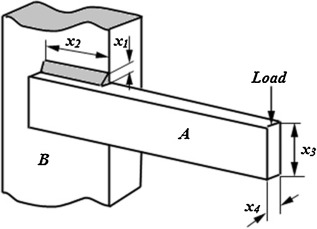
\includegraphics[scale=0.7]{img/Problems/WB.jpg}
    \end{center}
    \captionsetup{justification=centering}
    \caption{Schematic view of the welded beam design problem.}\label{fig:WB}
\end{figure}


We compare the results obtained by C-ITGO against a number of state-of-the-art methods used to solve this problem, including PSO-DE, HPSO, UPSO, MBA, CMA-ES, MVDE, CPSO, LCA, IPSO, CB-ABC, DELC, IABC-MAL, NM-PSO, APSO, WCA, IAPSO and SAMP-Jaya. Table \ref{tab:WB} shows the comparison of the statistical results obtained by all cited methods to solve the welded beam design problem. All the methods, with exception of CMA-ES, SAMP-Jaya and C-ITGO, took more than 10,000 iterations to achieve good quality solutions. C-ITGO achieved optimal solutions with a very small standard deviation of 3.65E-12, using ten times fewer function evaluations on average than most of the methods.

We write the statistics for the C-ITGO method in bold simply to highlight the reported results, not because it always presents the best statistics for all problems.


\begin{table*}[h]
    \tiny
\begin{center}

\begin{tabular}{ P{2.0cm} P{2.0cm} P{2.0cm} P{2.0cm} P{2.0cm} P{2.0cm} P{2.0cm} P{2.0cm}  }
\hline
\textbf{Method} & \textbf{Best} & \textbf{Mean} & \textbf{Worst} & \textbf{SD} & \textbf{MNFEs} \\
\hline
PSO-DE & 1.724852 & 1.724852 & 1.724852 & 6.70E-16 & 66,600 \\
HPSO & 1.724852 & 1.814295 & 1.749040 & 4.01E-02 & 81,000 \\
UPSO & 1.921990 & 2.837210 & N/A & 6.83E-01 & 100,000 \\
MBA & 1.724853 & 1.724853 & 1.724853 & 6.94E-19 & 47,340 \\
CMA-ES & 1.7248523 & 1.7248523 & 1.7248523 & 1.66E-09 & 4,658 \\
MVDE & 1.7248527 & 1.7248621 & 1.7249215 & 7.88E-06 & 15,000 \\
CPSO & 1.728024 & 1.748831 & 1.782143 & 1.29E-02 & 240,000 \\
LCA & 1.7248523 & 1.7248523 & 1.7248523 & 7.11E-15 & 15,000 \\
IPSO & 1.724852 & 1.7248787 & 1.7250002 & 3.28E-05 & 20,000 \\
CB-ABC & 1.724852 & 1.724852 & N/A & 2.38E-11 & 15,000 \\
DELC & 1.724852 & 1.724852 & 1.724852 & 4.10E-13 & 20,000 \\
IABC-MAL & 1.724852 & 1.724852 & 1.724852 & 2.31E-12 & 15,000 \\
NM-PSO & 1.724717 & 1.726373 & 1.733393 & 3.50E-03 & 80,000 \\
APSO & 1.736193 & 1.877851 & 1.993999 & 0.076118 & 50,000 \\
WCA & 1.724856 & 1.726427 & 1.744697 & 4.29E-03 & 46,450 \\
IAPSO & 1.7248523 & 1.7248528 & 1.7248624 & 2.02E-06 & 12,500 \\
SAMP-Jaya & 1.724852 & 1.724852 & 1.724852 & 6.7E-16 & 3,618.25 \\
\textbf{C-ITGO} & \bf{1.7248523} & \bf{1.7248523} & \bf{1.7248523} & \bf{3.65E-12} & \bf{940.68} \\


\hline
\end{tabular}
\end{center}
\vspace*{-6mm}
\caption{Statistical results of different methods for the Welded beam problem. \\[1em]}
\label{tab:WB}
\end{table*}



The results for C-ITGO and SAMP-Jaya are very similar, with the former having a slightly worse standard deviation, but converging in less than one-third of the number of function evaluations. We note here that the best solution achieved by NM-PSO is slightly unfeasible, so it should not be directly compared to the other methods.




\subsection{Tension/compression spring design problem}


% !TEX root = ../ITGO.tex

%\subsection*{Tension/compression spring design problem}


This problem was introduced by \cite{TC}, and the objective is the minimization of the weight of a tension/compression spring (Figure \ref{fig:TC}). The problem has three continuous design variables, being them the diameter of spring wire ($x_1 = D$), the diameter of spring mean coil ($x_2 = d$) and the number of active coils ($x_3 = P$). It is subject to three nonlinear and one linear inequality constraints. The objective function value at the known global optimum is $f(\bm{x}^*) = 0.01266523$. %The full mathematical formulation of the problem follows:

%\vspace{-0.5cm}

%\begin{align*}
\textbf{Minimize:} & \\
& f(\bm{x}) = (x_3 + 2)x_2x_1^2 \\[0.5em]
\textbf{subject to:} &\\
& g_1(\bm{x}) = 1 - \frac{x_2^3 x_3}{7.1785 x_1^4} \leq 0 \\
& g_2(\bm{x}) = \frac{4x_2^2 - x_1 x_2}{12,566 (x_2 x_1^3) - x_1^4} + \frac{1}{5.108 x_1^2} - 1 \leq 0 \\
& g_3(\bm{x}) = 1 - \frac{140.45 x_1}{x_2^2 x_3} \leq 0 \\
& g_4(\bm{x}) = \frac{x_2 + x_1}{1.5} - 1 \leq 0 \\[0.5em]
\textbf{with bounds:} & \\
& 0.05 \leq x_1 \leq 2, \quad 0.25 \leq x_2 \leq 1.3, \quad 2 \leq x_3 \leq 15
\end{align*}

\vspace{0.5cm}


\begin{figure}[h]
\begin{center}
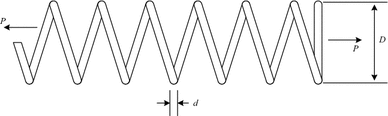
\includegraphics[scale=0.5]{img/Problems/TC.png}
\end{center}
\captionsetup{justification=centering}
\caption{Schematic view of the tension/compression spring design problem.}\label{fig:TC}
\end{figure}



A variety of methods were used in literature to solve the tension/compression spring design problem. Between them, we can cite CPSO, HPSO, NM-PSO, MBA, UPSO, PSO-DE, LCA, CB-ABC, QPSO, G-QPSO, APSO, CMA-ES, MVDE, DELC, WCA, IPSO, IAPSO, IABC-MAL and SAMP-Jaya. Table \ref{tab:TC} shows the statistical results of all methods, along with the number of function evaluations taken to achieve such results.


\begin{table*}[h]
    \tiny
\begin{center}

\begin{tabular}{ P{2.0cm} P{2.0cm} P{2.0cm} P{2.0cm} P{2.0cm} P{2.0cm} P{2.0cm} P{2.0cm}  }
\hline
\textbf{Method} & \textbf{Best} & \textbf{Mean} & \textbf{Worst} & \textbf{SD} & \textbf{MNFEs} \\
\hline


CPSO & 0.0126747 & 0.012730 & 0.012924 & 5.20E-04 & 240,000 \\
HPSO & 0.012665 & 0.012719 & 0.012707 & 1.58E-05 & 81,000 \\
NM-PSO & 0.012630 & 0.012633 & 0.012631 & 8.47E-07 & 80,000 \\
MBA & 0.012665 & 0.012713 & 0.012900 & 6.30E-05 & 7,650 \\
UPSO & 0.013120 & 0.022940 & N/A & 7.20E-03 & 100,000 \\
PSO-DE & 0.012665 & 0.012665 & 0.012665 & 1.20E-08 & 24,950 \\
LCA & 0.01266523 & 0.01266541 & 0.01266667 & 3.88E-07 & 15,000 \\
CB-ABC & 0.012665 & 0.012671 & N/A & 1.42E-05 & 15,000 \\
QPSO & 0.012669 & 0.018127 & 0.013854 & 1.34E-03 & 2,000 \\
G-QPSO & 0.012665 & 0.017759 & 0.013524 & 1.27E-03 & 2,000 \\
APSO & 0.012700 & 0.013297 & 0.014937 & 6.85E-04 & 120,000 \\
CMA-ES & 0.01266524 & 0.01266861 & 0.01269335 & 6.30E-06 & 19,445 \\
MVDE & 0.01266527 & 0.01266732 & 0.01271906 & 2.45E-06 & 10,000 \\
DELC & 0.012665 & 0.012666 & 0.012665 & 1.30E-07 & 20,000 \\
WCA & 0.012665 & 0.012746 & 0.012952 & 8.06E-05 & 11,750 \\
IPSO & 0.01266567 & 0.012671486 & 0.01268312 & 3.89E-06 & 20000 \\
IAPSO & 0.01266523 & 0.013676527 & 0.01782864 & 1.573E-3 & 2,000 \\
IABC-MAL & 0.01266523 & 0.01266525 & 0.01266539 & 6.78E-08 & 15,000 \\
SAMP-Jaya & 0.012664 & 0.013193 & 0.012714 & 9.25E-05 & 6,861 \\
\textbf{C-ITGO} & \bf{0.01266523} & \bf{0.01266523} & \bf{0.01266525} & \bf{2.81E-9} & \bf{535.08} \\

\hline
\end{tabular}
\end{center}
\vspace*{-6mm}
\caption{Statistical results of different methods for tension/compression spring design problem. \\[1em]}
\label{tab:TC}
\end{table*}




The methods vary greatly in the number of function evaluations required to converge to good quality solutions. Only three of the methods (QPSO, G-QPSO and IAPSO) achieved convergence with 2,000 function evaluations, while some methods required more than 100,000. The best solution achieved by all methods have the same fitness value up to five decimal places, with the exception of CPSO, UPSO, APSO and NM-PSO.
 
The best solution reported by NM-PSO is again unfeasible, so we do not compare it against other methods. The SAMP-Jaya method also seems to report a slightly unfeasible best solution, differing from the optimal value reported by other methods. However, the result achieved by SAMP-Jaya differs only at the sixth decimal place, and the difference may be due to wrong rounding. We cannot state this for sure since we do not have access to the solution vector found by the method. Given the differences between the precision in the solutions reported by the methods, we consider $f(\bm{x}) = 0.012665$ to be the fitness at the global optimum.

The C-ITGO method performed remarkably well on this problem, converging to the best solution found in 535.08 function evaluations on average, almost four times less than the second best competing method. Also, the standard deviation is very small, in the order of 2.81E-9. 

Given the relatively small domain of the problem, we believe that the C-ITGO method was able to cover the space efficiently, providing hot starting points for the local search method, which proved to be very effective in this case.




\subsection{Three-bar truss design problem}

% !TEX root = ../ITGO.tex

%\subsection*{Three-bar truss design problem}

The three-bar truss design problem \cite{TB} consists in minimizing the volume of a statically loaded three-bar truss. There are two continuous design variables and three nonlinear inequality constraints, based on the stress on each of the truss members ($\sigma$), with $f(\bm{x}^*) = 263.895843$. Figure \ref{fig:TB} shows the schematic view of the problem. %The full problem statement follows:

%\vspace{-0.5cm}

%\begin{align*}
\textbf{Minimize:} & \\
& f(\bm{x}) = 2 \sqrt{2} x_1 + l x_2\\[0.5em]
\textbf{subject to:} &\\
& g_1(\bm{x}) = \frac{\sqrt{2} x_1 + x_2}{\sqrt{2} x_1^2 + 2 x_1 x_2} P - \sigma \leq 0 \\
& g_2(\bm{x}) = \frac{x_2}{\sqrt{2} x_1^2 + 2 x_1 x_2} P - \sigma \leq 0 \\
& g_3(\bm{x}) = \frac{1}{\sqrt{2} x_2 + x_1 x_2} P - \sigma \leq 0 \\[0.5em]
\textbf{where:} & \\
& l = 100cm, \quad P = 2 kN/cm^2, \quad \sigma = 2 kN/cm^2 \\[0.5em]
\textbf{with bounds:} & \\
& 0 \leq x_1, x_2 \leq 1
\end{align*}

\vspace{0.5cm}


\begin{figure}[h]
    \begin{center}
    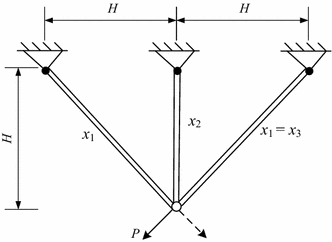
\includegraphics[scale=0.5]{img/Problems/TB.png}
    \end{center}
    \captionsetup{justification=centering}
    \caption{Schematic view of the three-bar truss design problem.}\label{fig:TB}
\end{figure}



Here we present only the five best-performing methods used to solve this problem since the solutions found in the literature have very small variance from each other. These methods are PSO-DE, CMA-ES, MVDE, DELC, MBA and IABC-MAL. We present the statistical results for this problem in Table \ref{tab:TB}.


\begin{table*}[h]
    \tiny
\begin{center}

\begin{tabular}{ P{2.0cm} P{2.0cm} P{2.0cm} P{2.0cm} P{2.0cm} P{2.0cm} P{2.0cm} P{2.0cm}  }
\hline
\textbf{Method} & \textbf{Best} & \textbf{Mean} & \textbf{Worst} & \textbf{SD} & \textbf{MNFEs} \\
\hline

PSO-DE & 263.895843 & 263.895843 & 263.895843 & 4.50E-12 & 17,600 \\
CMA-ES & 263.895843 & 263.895843 & 263.895843 & 2.7E-09 & 1,706 \\
MVDE & 263.895843 & 263.895843 & 263.895855 & 2.58E-07 & 7,000 \\
DELC & 263.895843 & 263.895843 & 263.895843 & 4.3E-14 & 10,000 \\
MBA & 263.895852 & 263.897996 & 263.915983 & 3.93E-03 & 13,280 \\
IABC-MAL & 263.895843 & 263.895843 & 263.895843 & 0.0 & 15,000 \\
\textbf{C-ITGO} & \bf{263.895843} & \bf{263.895843} & \bf{263.895843} & \bf{2.0E-12} & \bf{136.48} \\


\hline
\end{tabular}
\end{center}
\vspace*{-6mm}
\caption{Statistical results of different methods for three-bar truss design problem. \\[1em]}
\label{tab:TB}
\end{table*}



From Table \ref{tab:TB} it is possible to note that all methods have very similar results, differing mainly in the number of function calls. This is not surprising, given that the problem is simpler, has fewer variables and consequently has a smaller domain than any other engineering design problem considered in this work.

C-ITGO achieved convergence quickly, taking 136.48 function evaluations on average. In this problem, we have set a small population, as well as a small number of function calls allowed in the local search procedure. Thus, we obtained the lowest MNFEs than any of the competing techniques, at least ten times lower. It seems that the solutions found by the topographical heuristic were already close to the optimum, so the local search converged in very few iterations. However, the C-ITGO method has a slightly worse standard deviation than DELC and IABC-MAL.



\subsection{Speed reducer design problem}

% !TEX root = ../ITGO.tex

%\subsection*{Speed reducer design problem}

In this problem, the total weight of the speed reducer (Figure \ref{fig:SR}) is to be minimized. The problem has seven design variables: face width ($b$), teeth module ($m$), number of teeth on the pinion ($z$), first and second length of shafts between bearings ($l_1$ and $l_2$) and first and second shafts diameter ($d_1$ and $d_2$) \cite{SR}. The problem has 11 nonlinear constraints, and the third variable is constrained to be an integer. A second version of the problem is also found in literature, where the only difference is in the lower bound of the fifth variable (7.8 for SR1 and 7.3 for SR2). The objective function value at the optimal is $f(\bm{x}^*) = 2996.34816497$ for the first version (SR1), and $f(\bm{x}^*) = 2994.471066$ for the second version (SR2). %The mathematical formulation of the problem follows:

%\vspace{-0.5cm}

%\begin{align*}
\textbf{Minimize:} & \\
& f(\bm{x}) = 0.7854x_1x_2^2(3.333x_3^2 + 14.9334x_3 - 43.0934) \\
& \quad \qquad - 1.508x_1(x_6^2 + x_7^2) + 7.4777(x_6^3 + x_7^3) \\
& \quad \qquad + 0.7854(x_4 x_6^2 + x_5x_7^2) \\[0.5em]
\textbf{subject to:} &\\
& g_1(\bm{x}) = \frac{27}{x_1x_2^2x_3} - 1 \leq 0 \\
& g_2(\bm{x}) = \frac{397.5}{x_1x_2x_3^2} - 1 \leq 0 \\
& g_3(\bm{x}) = \frac{1.93x_4^3}{x_2x_3x_6^4} -1 \leq 0 \\
& g_4(\bm{x}) = \frac{1.93x_5^3}{x_2x_3x_7^4} -1 \leq 0 \\
& g_5(\bm{x}) = \frac{1}{110x_6^3} \sqrt{\Big( \frac{745x_4}{x_2x_3} \Big)^2 + 16.9 \times 10^6} - 1 \leq 0 \\
& g_6(\bm{x}) = \frac{1}{85x_7^3} \sqrt{\Big( \frac{745x_5}{x_2x_3} \Big)^2 + 157.5 \times 10^6} - 1 \leq 0 \\
& g_7(\bm{x}) = \frac{x_2x_3}{40} - 1 \leq 0 \\
& g_8(\bm{x}) = \frac{5x_2}{x_1} - 1 \leq 0 \\
& g_9(\bm{x}) = \frac{x_1}{12x_2} - 1 \leq 0 \\
& g_{10}(\bm{x}) = \frac{1.5x_6 + 1.9}{x_4} - 1 \leq 0 \\
& g_{11}(\bm{x}) = \frac{1.1x_7 + 1.9}{x_5} - 1 \leq 0 \\[0.5em]
\textbf{with bounds:} & \\
& 2.6 \leq x_1 \leq 3.6, \quad 0.7 \leq x_2 \leq 0.8, \quad 17 \leq x_3 \leq 28, \quad x_3 \in \mathbb{Z} \\
& 7.3 \leq x_4 \leq 8.3, \quad 7.8 \leq x_5 \leq 8.3 \ (\text{or} \ 7.3 \leq x_5 \leq 8.3) \\
& 2.9 \leq x_6 \leq 3.9, \quad 5.0 \leq x_7 \leq 5.5
\end{align*}

\vspace{0.5cm}

\begin{figure}[h]
    \begin{center}
    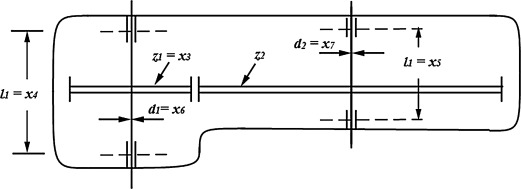
\includegraphics[scale=0.5]{img/Problems/SR.jpg}
    \end{center}
    \captionsetup{justification=centering}
    \caption{Schematic view of the speed reducer design problem.}\label{fig:SR}
\end{figure}



For SRI, we compare C-ITGO results against four optimization methods, namely LCA, IPSO, APSO and IAPSO, shown in Table \ref{tab:SP1}.

The LCA, IPSO, IAPSO and C-ITGO present similar results, all finding the constrained global optimum solution and having very low standard deviation.



\begin{table*}[h]
    \tiny
    \begin{center}
    
    \begin{tabular}{ P{2.0cm} P{2.0cm} P{2.0cm} P{2.0cm} P{2.0cm} P{2.0cm} P{2.0cm} P{2.0cm}  }
    \hline
    \textbf{Method} & \textbf{Best} & \textbf{Mean} & \textbf{Worst} & \textbf{SD} & \textbf{MNFEs} \\
    \hline
    
    LCA & 2996.34816497 & 2996.34816497 & 2996.34816497 & 2.63E-12 & 24,000 \\
    IPSO & 2996.34816497 & 2996.3481 & 2996.34816509 & 2.43E-18 & 20,000 \\
    APSO & 3177.530771 & 3855.581557 & 4677.005187 & 473.767 & 30,000 \\  
    IAPSO & 2996.34816497 & 2996.34816497 & 2996.34816497 & 6,88E-13 & 6,000 \\
    \textbf{C-ITGO} & \bf{2996.34816497} & \bf{2996.34816497} & \bf{2996.34816497} & \bf{7.5E-13} & \bf{856.40} \\
        
    \hline
    \end{tabular}
    \end{center}
    \vspace*{-6mm}
    \caption{Statistical results of different methods for the speed reducer design problem I. \\[1em]}
    \label{tab:SP1}
    \end{table*}
    
    

The first three methods take at least 20,000 iterations to converge to good quality solutions, while IAPSO takes only 6,000 NFEs. C-ITGO outperforms the other methods by a large margin, converging in 858.40 function calls on average while maintaining negligible higher standard deviation than IAPSO and IPSO.

For this problem, we used considerably greater populations, of sizes 150 ($PS_1$) and 10 ($PS_2$), while maintaining the number of allowed function evaluations of the local search relatively small (100 and 200). For the worst case, C-ITGO took 3 full iterations to converge, while in most cases it converged in the first iteration.

For SRII, the methods used for comparison were PSO-DE, WCA, DELC, CB-ABC, CMA-ES, MVDE, IABC-MAL, LCA, APSO, MBA, IPSO, IAPSO and SAMP-Jaya. The reported results for the SAMP-Jaya method seems to violate the integer constraint at variable three, but it is included to show that even in harder situations the C-ITGO algorithm can still produce state-of-the-art results.

From Table \ref{tab:SP2}, we can see that DELC, CMA-ES, MVDE, IABC-MAL, LCA, IAPSO, SAMP-Jaya and C-ITGO are the only methods that converged to the optimum in every run, having very small standard deviation. Although similar results are observed regarding the quality of the solutions, C-ITGO converges much faster than any competing method, using seven times fewer function evaluations than SAMP-Jaya. The standard deviation achieved by C-ITGO is also only worse than the standard deviation reported by IABC-MAL (the difference is in the order of 1E-13), which took 15,000 function evaluations to converge.


\begin{table*}[h]
    \tiny
    \begin{center}
    
    \begin{tabular}{ P{2.0cm} P{2.0cm} P{2.0cm} P{2.0cm} P{2.0cm} P{2.0cm} P{2.0cm} P{2.0cm}  }
    \hline
    \textbf{Method} & \textbf{Best} & \textbf{Mean} & \textbf{Worst} & \textbf{SD} & \textbf{MNFEs} \\
    \hline
    
    PSO-DE & 2996.348167 & 2996.348174 & 2996.348204 & 6.40E-06 & 54,350 \\
    WCA & 2994.471066 & 2994.474392 & 2994.505578 & 7.4E-03 & 15,150 \\    
    DELC & 2994.471066 & 2994.471066 & 2994.471066 & 1.90E-12 & 30,000 \\
    CB-ABC & 2994.471066 & 2994.471066 & N/A & 2.48E-07 & 15,000 \\
    CMA-ES & 2994.471066 & 2994.471066 & 2994.471066 & 8.98E-10 & 12,998 \\
    MVDE & 2994.471066 & 2994.471066 & 2994.471066 & 2.82E-07 & 30,000 \\    
    IABC-MAL & 2994.471066 & 2994.471066 & 2994.471066 & 8.51E-13 & 15,000 \\ 
    LCA & 2994.471066 & 2994.471066 & 2994.471066 & 2.66E-12 & 24000 \\
    APSO & 3187.630486 & 3822.640624 & 4443.017639 & 366.146 & 30,000 \\
    MBA & 2994.482453 & 2996.769019 & 2999.652444 & 1.56 & 6300 \\
    IPSO & 2994.471067 & 2994.47108 & 2994.4711 & 9.27E-06 & 20,000 \\
    IAPSO & 2994.471066 & 2994.471066 & 2994.471066 & 2.65E-09 & 6,000 \\
    SAMP-Jaya & 2760.673988 & 2760.673988 & 2760.673988 & 2.54E-11 & 3744.66 \\    
    \textbf{C-ITGO} & \bf{2994.471066} & \bf{2994.471066} & \bf{2994.471066} & \bf{9.28E-13} & \bf{491.24} \\ 
    
  

    \hline
    \end{tabular}
    \end{center}
    \vspace*{-6mm}
    \caption{Statistical results of different methods for the speed reducer design problem II. \\[1em]}
    \label{tab:SP2}
    \end{table*}
    
    

For this specific problem, we used the SQP algorithm as local search and rounded the value of the third variable. In this case, this approach proved to converge much faster than using a mixed integer local search. Also, the first population size is considerably smaller than the one used in SRI (100 in this problem).



\subsection{Pressure vessel design problem}

% !TEX root = ../ITGO.tex

%\subsection*{Pressure vessel design problem}

In the pressure vessel design problem, the objective is to minimize the total manufacturing cost, including the cost of the material, forming and welding costs \cite{PV}. The problem is subject to three linear and one nonlinear inequality constraint, and its structure is shown in Figure \ref{fig:PV}. The four variables are the thickness of the shell ($x_1 = T_s$), the thickness of the head ($x_2 = T_h$), the inner radius ($x_3 = R$), and the length of the cylindrical section of the vessel ($x_4 = L$). This is an example of a mixed integer problem, where the first and second variables are constrained to be integers. The value of the objective function at the best known feasible solution is around $f(\bm{x}^*) = 6059.7143$. %The mathematical formulation for the pressure vessel problem can be expressed as follows:

%\vspace{-0.5cm}

%\begin{align*}
\textbf{Minimize:} & \\
& f(\bm{x}) = 0.6224z_1x_3x_4 + 1.7781z_2x_3^2 + 3.1661z_1^2x_4 + 19.84z_1^2x_3 \\[0.5em]
\textbf{subject to:} &\\
& g_1(\bm{x}) = -z_1 + 0.193x_3 \leq 0 \\
& g_2(\bm{x}) = -z_2 + 0.00954x_3 \leq 0 \\
& g_3(\bm{x}) = -\pi x_3^2x_4^2 - \frac{4}{3} \pi x_3^3 + 1,296,000 \leq 0 \\
& g_4(\bm{x}) = x_4 - 240  \leq 0 \\[0.5em]
\textbf{where:} & \\
& z_1 = 0.0625x_1 \\
& z_2 = 0.0625x_2 \\[0.5em]
\textbf{with bounds:} & \\
& 1 \leq x_1, x_2 \leq 99, \quad 10 \leq x_2, x_3 \leq 200, \quad x_1, x_2 \in \mathbb{Z}
\end{align*}

\vspace{0.5cm}

\begin{figure}[h]
    \begin{center}
    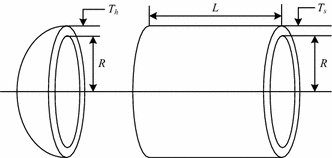
\includegraphics[scale=0.4]{img/Problems/PV.png}
    \end{center}
    \captionsetup{justification=centering}
    \caption{Schematic view of pressure vessel design problem.}\label{fig:PV}
\end{figure}



We compare C-ITGO against the UPSO, QPSO, G-QPSO, CMA-ES, MVDE, CB-ABC, PSO-DE, HPSO, WCA, LCA, APSO, CPSO, MBA, IPSO, DELC, IABC-MAL, SAMP-Jaya and IAPSO methods. The statistical results are shown in Table \ref{tab:PV}. Some of the methods used to solve this problem report unfeasible results (PSO-DE, WCA, MBA and SAMP-Jaya), probably either because the integer constraints are ignored or due to wrong rounding. Nevertheless, we still use the results of these methods to prove the superior convergence of C-ITGO, even in constrained mixed integer problems.



\begin{table*}[h]
    \tiny
    \begin{center}
    
    \begin{tabular}{ P{2.0cm} P{2.0cm} P{2.0cm} P{2.0cm} P{2.0cm} P{2.0cm} P{2.0cm} P{2.0cm}  }
    \hline
    \textbf{Method} & \textbf{Best} & \textbf{Mean} & \textbf{Worst} & \textbf{SD} & \textbf{MNFEs} \\
    \hline
    
    UPSO & 6544.2700 & 9032.5500 & N/A & 9.95E+02 & 100,000 \\
    QPSO & 6059.7209 & 8017.2816 & 6440.3786 & 4.79E+02 & 8,000 \\
    G-QPSO & 6059.7208 & 7544.4925 & 6440.3786 & 4.48E+02 & 8,000 \\
    CMA-ES & 6059.7143 & 6170.25055 & 6410.08676 & 140.4843 & 30,018 \\
    MVDE & 6059.7144 & 6059.99724 & 6090.53353 & 2.9103 & 15,000 \\ 
    CB-ABC & 6059.7143 & 6126.6237 & N/A & 1.14E+02 & 15,000 \\
    PSO-DE & 6059.7140 & 6059.7140 & N/A & N/A & 42,100 \\
    HPSO & 6059.7143 & 6099.9323 & 6288.6770 & 86.2000 & 81,000 \\
    WCA & 5885.3327 & 6198.6172 & 6590.2129 & 213.0490 & 27,500 \\
    LCA & 6059.8553 & 6070.5884 & 6090.6114 & 11.37534 & 24,000 \\
    APSO & 6059.7242 & 6470.7156 & 7544.4927 & 326.9688 & 200,000 \\
    CPSO & 6061.0777 & 6147.1332 & 6363.8041 & 86.4500 & 240,000 \\
    MBA & 5889.3216 & 6200.64765 & 6392.5062 & 160.34 & 70,650 \\    
    IPSO & 6059.7143 & 6059.7155 & 6059.7257 & 0.00232 & 20,000 \\
    DELC & 6059.7143 & 6059.7143 & 6059.7143 & 2.10E-11 & 30,000 \\  
    IABC-MAL & 6059.7143 & 6072.5972 & 6089.2720 & 1.88E-06 & 15,000 \\
    SAMP-Jaya & 5872.2129 & 5872.2129 & 5872.2129 & 5.0E-12 & 6513.33 \\    
    IAPSO & 6059.7143 & 6068.7539 & 6090.5314 & 14.0057 & 7,500 \\
    \textbf{C-ITGO} & \bf{6059.7143} & \bf{6059.7143} & \bf{6059.7143} & \bf{9.8E-13} & \bf{1101.64} \\
    
    \hline
    \end{tabular}
    \end{center}
    \vspace*{-6mm}
    \caption{Statistical results of different methods for the pressure vessel design problem. \\[1em]}
    \label{tab:PV}
    \end{table*}
    
    


The algorithms CMA-ES, CB-ABC, HPSO, IABC-MAl, IPSO, DELC, IAPSO and C-ITGO are the only who found the feasible optimal solution. All other methods presented relatively poor performance, with much higher NFEs on average. C-ITGO takes less than five times the number of function evaluations to converge than the best competing method, SAMP-Jaya, which reported a result of 6513.33 MNFEs. Also, C-ITGO achieves the smallest standard deviation among all methods. All runs of C-ITGO converged quickly to the known global optimum, showing unarguably better results than any other method compared in this problem.



\subsection{Gear train design problem}

% !TEX root = ../ITGO.tex

In this problem, the objective is to minimize the cost of the gear ratio of the gear train \cite{PV}. An example is shown in Figure \ref{fig:GT}. The problem has four variables, representing the number of teeth for the four gears ($x_1 = A$, $x_2 = B$, $x_3 = D$, and $x_4 = F$), with $f(\bm{x}^*) = 2.700857E \! - \! 12$. The only constraint of the problem is that all variables must be integers. %The full problem statement follows:

%\vspace{-0.5cm}

%\begin{align*}
\textbf{Minimize:} & \\
& f(\bm{x}) = \Big(\Big(\frac{1}{6.931}\Big) - \Big(\frac{x_2 x_3}{x_1 x_4} \Big)  \Big)^2 \\[0.5em]
\textbf{with bounds:} & \\
& 12 \leq x_i \leq 60, \quad i = 1, 2, 3, 4 \\
& x_i \in \mathbb{Z}, \quad i = 1, 2, 3, 4
\end{align*}

\vspace{0.5cm}


\begin{figure}[h]
    \begin{center}
    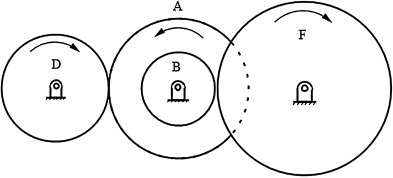
\includegraphics[scale=0.5]{img/Problems/GT.jpg}
    \end{center}
    \captionsetup{justification=centering}
    \caption{Gear train design problem structure.}\label{fig:GT}
\end{figure}



We compare the C-ITGO results, shown in Table \ref{fig:GT}, against other five methods: MBA, UPSO, CS, APSO and IAPSO. In general, all methods compared achieved similar results, having found the global optimal solution for the problem. The main difference relies on the number of function calls, varying from 100,000 for UPSO to 800 for IAPSO.


\begin{table*}[h]
    \tiny
\begin{center}

\begin{tabular}{ P{2.0cm} P{2.0cm} P{2.0cm} P{2.0cm} P{2.0cm} P{2.0cm} P{2.0cm} P{2.0cm}  }
\hline
\textbf{Method} & \textbf{Best} & \textbf{Mean} & \textbf{Worst} & \textbf{SD} & \textbf{MNFEs} \\
\hline

MBA & 2.700857E-12 & 2.062904E-08 & 2.47E-09 & 3.94E-09 & 1,120 \\
UPSO & 2.700857E-12 & 3.80562E-08 & N/A & 1.09E-07 & 100,000 \\
CS & 2.7009E-12 & 1.9841E-9 & 2.3576E-9 & 3.55E-9 & 5,000 \\
APSO & 2.700857E-12 & 4.781676E-07 & 7.072678E-06 & 1.44E-06 & 8,000 \\
IAPSO & 2.700857E-12 & 5.492477E-09 & 1.827380E-08 & 6.36E-09 & 800 \\
\textbf{C-ITGO} & \bf{2.700857E-12} & \bf{4.6504232E-09} & \bf{2.7264505E-08} & \bf{6.85E-09} & \bf{773.0} \\


\hline
\end{tabular}
\end{center}
\vspace*{-6mm}
\caption{Statistical results of different methods for the gear train design problem. \\[1em]}
\label{tab:GT}
\end{table*}




Since this is an integer optimization problem, we used the mixed integer local search based on the NOMAD solver. In this problem, the solver had some difficulty in some runs, achieving 6.85E-09 of standard deviation, more than IAPSO, CS and MBA. The mean fitness value, however, is just worse than the CS method, which takes 5,000 function calls to converge. Besides this drawbacks, C-ITGO was the fastest method to achieve convergence, taking only 773.0 function calls on average.



\subsection{Multiple disk clutch brake design problem}

% !TEX root = ../ITGO.tex

%\subsection*{Multiple disk clutch brake design problem}

This is also an example of a problem where all variables are discrete. The Multiple disk clutch brake design problem aims at minimizing the mass of a multiple disk clutch brake \cite{MD}. There are five integer variables: the inner radius ($x_1$), outer radius ($x_2$), thickness of the disk ($x_3$), actuating force ($x_4$) and number of friction surfaces ($x_5$) (Figure \ref{fig:MD}). The problem is also constrained by nine nonlinear inequalities. The objective function at the optimal solution is $f(\bm{x}^*) = 0.313656$. %The mathematical formulation of the problem follows:

%\vspace{-0.5cm}

%\begin{align*}
\textbf{Minimize:} & \\
& f(\bm{x}) = \pi(x_2^2 - x_1^2) x_3 (x_5 + 1) \rho \\[0.5em]
\textbf{subject to:} & \\
& g_1(\bm{x}) = x_2 - x_1 - \Delta R \geq 0 \\
& g_2(\bm{x}) = L_{max} - (x_5 + 1) (x_3 + \delta) \geq 0 \\
& g_3(\bm{x}) = p_{max} - p_{rz} \geq 0 \\
& g_4(\bm{x}) = p_max * Vsr_{max} - p_{rz} * Vsr \geq 0 \\
& g_5(\bm{x}) = Vsr_{max} - Vsr \geq 0 \\
& g_6(\bm{x}) = T_{max} - T \geq 0 \\
& g_7(\bm{x}) = M_h - s  M_s \geq 0 \\
& g_7(\bm{x}) = T \geq 0 \\[0.5em]
\textbf{where:} & \\
& M_h = \frac{2}{3} \mu x_4 x_5 \frac{x_2^3 - x_1^3}{x_2^2 - x_1^2} N \cdot mm  \\
& \omega = \frac{\pi n}{30} rad/s  \\
& A = \pi (x_2^2 - x_1^2) mm^2  \\
& p_{rz} = \frac{x_4}{A} N/mm^2 \\
& V_{sr} = \frac{pi R_{sr} n}{30} mm /s \\
& R_{sr} = \frac{2}{3} \frac{x_2^3 - x_1^3}{x_2^2 x_1^2} mm \\
& \Delta R = 20mm, \quad L_{max} = 30mm, \quad \mu = 0.6 \\
& p_{max} = 1MPa, \quad \rho = 0.0000078kg/mm^3 \\
& Vsr_{max} = 10m/s, \quad \delta = 0.5mm, \quad s = 1.5; \\
& T_{max} = 15s, \quad n = 250rpm, \quad I_{z} = 55Kg \cdot m^2 \\
& M_s = 40Nm, \quad Mf = 3Nm \\[0.5em]
\textbf{with bounds:} & \\
& 60 \leq x_1 \leq 80, \quad 90 \leq x_2 \leq 110, \quad 1 \leq x_3 \leq 3 \\
& 0 \leq x_4 \leq 1000, \quad 2 \leq x_5 \leq 9 \\
& x_i \in \mathbb{Z}, \quad i = 1, 2, 3, 4, 5
\end{align*}

\vspace{0.5cm}


\begin{figure}[h]
    \begin{center}
    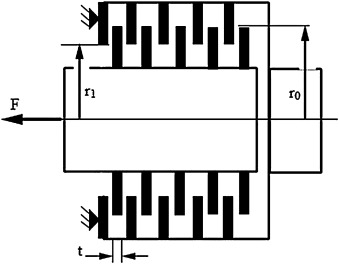
\includegraphics[scale=0.5]{img/Problems/MD.jpg}
    \end{center}
    \captionsetup{justification=centering}
    \caption{Schematic view of the multiple disk clutch brake design problem.}\label{fig:MD}
\end{figure}


To compare the results, we used only methods who achieved close performance to the obtained by C-ITGO, since some methods in literature have very diverging results. The methods compared are WCA, IPSO, APSO and IAPSO. The WCA, IPSO, and IAPSO methods achieved good performance in this problem, finding the global optimal solution and having very small variance, as shown in Table \ref{tab:MD}. The WCA and IAPSO took very few function evaluations to converge, respectively 500 and 400. IPSO took long more, with 20,000 function evaluations. However, the reported standard deviation for IPSO was 0.0.


\begin{table*}[h]
    \tiny
    \begin{center}
    
    \begin{tabular}{ P{2.0cm} P{2.0cm} P{2.0cm} P{2.0cm} P{2.0cm} P{2.0cm} P{2.0cm} P{2.0cm}  }
    \hline
    \textbf{Method} & \textbf{Best} & \textbf{Mean} & \textbf{Worst} & \textbf{SD} & \textbf{MNFEs} \\
    \hline

    WCA & 0.313656 & 0.313656 & 0.313656 & 1.69E-16 & 500 \\
    IPSO & 0.313656 & 0.313656 & 0.313656 & 0.0 & 20,000 \\
    APSO & 0.337181 & 0.506829 & 0.716313 & 0.09767 & 2,000 \\    
    IAPSO & 0.313656 & 0.313656 & 0.313656 & 1.13E-16 & 400 \\
    \textbf{C-ITGO} & \bf{0.313656} & \bf{0.313656} & \bf{0.313656} & \bf{1.13E-16} & \bf{286.48} \\

    \hline
    \end{tabular}
    \end{center}
    \vspace*{-6mm}
    \caption{Statistical results of different methods for the multiple disk clutch break design problem. \\[1em]}
    \label{tab:MD}
    \end{table*}
    
    

The C-ITGO clearly outperforms the other methods, having a standard deviation of 1.13E-16, while converging with only 286.48 function evaluations on average. For this problem, we used very small populations, of sizes 20 ($PS_1$) and 5 ($PS_2$). The number of function evaluations in the first step was 100, and most runs converged in much less, enjoying the quality of initial solutions provided by the topographical heuristic step. Some runs, however, took more than 1,000 function evaluations, bringing the mean NFEs up.



\subsection{Best Solutions to the Engineering Problems}

Table \ref{tab:BestResults} shows the fitness value, the values of the variables and the values of the constraints for the best solution found by C-ITGO for all problems. The precision of the results of each problem was set to match the results reported by the competing methods cited in this work. However, to the best of our knowledge, the best solution found by C-ITGO for each problem is equal to, or negligibly worse (up to several decimal places) than the best solutions reported by state-of-the-art methods.


\noindent
\begin{table*}[h]
    \tiny
\begin{center}
%\begin{adjustwidth}{-1cm}{}
\begin{tabular}{ | P{1.0cm} | P{1.2cm} |  P{1.2cm} | P{1.2cm} | P{1.2cm} | P{1.2cm} | P{1.2cm} | P{1.2cm} | P{1.2cm} |  }
\hline
\textbf{Prob.} & \textbf{WB} & \textbf{TC} & \textbf{TB} & \textbf{SRI} & \textbf{SRII} & \textbf{PV} & \textbf{GT} & \textbf{MD} \\
\hline
\rule{0pt}{3ex}
$f(\cdot)$ & 1.7248523 & 0.01266523 & 263.895843 & 2996.34816497 & 2994.471066 & 6059.7143 & 2.700857E-12 & 0.313656 \\
\hline
\rule{0pt}{3ex}
$\bm{x}_1$ &  0.2057296 & 0.05168906 & 0.788675 & 3.5 & 3.5 & 13.0 & 43 & 70  \\
$\bm{x}_2$ &  3.4704886 & 0.35671774 & 0.408248 & 7.0 & 0.7 & 7.0 & 16 & 90 \\
$\bm{x}_3$ &  9.0366239 & 11.28896574 & & 17 & 17 & 41.5984 & 19 &  1  \\
$\bm{x}_4$ &  0.2057296 & & & 7.3 & 7.3 & 176.6366 & 49 & 830  \\
$\bm{x}_5$ & & & & 7.8 & 7.715320 & & & 3 \\
$\bm{x}_6$ & & & & 3.35021467 & 3.350215 & & &   \\
$\bm{x}_7$ & & & & 5.28668323 & 5.286654 & & &   \\
\hline
\rule{0pt}{3ex}
$\bm{g}_1$ & 0.0 & 0.0 & 0.0 & -0.07391528 & -0.073915 & -2.6645E-15 & & 0.0  \\
$\bm{g}_2$ & 0.0 & 0.0 & -1.464102 & -0.19799853 & -0.197999 & -0.0359 & & -24.0  \\
$\bm{g}_3$ & 0.0 & -4.05378563 & -0.535898 & -0.49917225 & -0.499172 & -4.4238E-09 & & -0.917438 \\
$\bm{g}_4$ & -3.4329838 & -1.09159320 & & -0.90147170 & -0.904644 & -63.3634 & & -9.826183  \\
$\bm{g}_5$ & -0.0807296 & & & -8.846257E-13 & -2.220446E-16 & & &  -7.894697 \\
$\bm{g}_6$ & -0.2355403 & & & -4.885758E-12 & 0.0 & & & -0.173855  \\
$\bm{g}_7$ & -1.818989E-12 & & & -0.7025 & -0.7025 & & & -40.118750 \\
$\bm{g}_8$ & & & & -1.887379E-15 & 0.0 & & &  -14.826145 \\
$\bm{g}_9$ & & & & -0.58333333 & -0.583333 & & &    \\
$\bm{g}_{10}$ & & & & -0.05132575 & -0.051326 & & &    \\
$\bm{g}_{11}$ & & & & -0.01085237 & 0.0 & & &    \\
\hline
\end{tabular}
%\end{adjustwidth}
\end{center}
\vspace*{-6mm}
\caption{Results for the best solution found by C-ITGO for each engineering design problem. \\[1em]}
\label{tab:BestResults}
\end{table*}




\subsection{Statistical Tests To Analyse the Computational Results}

We now prove the significant improvement of C-ITGO over the competing methods by means of a nonparametric statistical test, where no assumptions are made regarding the underlying distribution of the data. Since no other algorithm than C-ITGO solves all the eight engineering design problems presented in this paper, we cannot apply typical statistical methods, such as the Friedman test \cite{Friedman}.

Instead, we use the Skillings-Mack test \cite{Skillings}, which is a Friedman\allowbreak-type statistical test that can be used when there are missing data, and that reduces to the Friedman test when the data has no missing entries. Just as in the Friedman test, the Skillings-Mack test finds the rank of the competing algorithms for each problem and then calculates the mean or average rank. The lower the mean rank, the better is the performance of the algorithm. The Skillings-Mack statistical test is also useful when there are many ties or equal ranks, as well as for small samples.

The method reports a \textit{p-value}, the probability that, when the null hypothesis is assumed to be true (in this case, no difference between the performance of the optimization methods), the results observed by the experiments at hand are at least of the same magnitude that the true values that would be observed in the limit of an infinite number of samples. Thus, a small p-value, say less than 0.05, represents a high chance that the null hypothesis is false.

In this work, the mean number of function evaluations (MNFEs) is used as the comparing metric. We used the \textit{Skillings.Mack} package \cite{SkillMack} of the \textit{R} language \cite{R} to report the following results.

In Table \ref{tab:SkillMack_3} we show the results of applying the statistical test to all the methods that solved at least three of the eight engineering design problems considered in this work. The mean rank of C-ITGO is 1.0, given that it has the smallest MNFEs for all problems. That is much less than IAPSO and SAMP-Jaya, which have a mean rank of 2.75. The mean ranks are also shown in the form of a bar plot for all methods in Figure \ref{fig:SkillMack_3}.


\begin{table}[h]
    \tiny
    \begin{center}
    
    \begin{tabular}{ | P{3.0cm} | P{3.0cm} | }

    \hline

    \rule{0pt}{3ex}
    \textbf{Algorithms} & \textbf{Skillings-Mack ranks}  \\
    \hline

    \rule{0pt}{3ex}
    C-ITGO & 1.0 \\[1em]

    \rule{0pt}{3ex}
    IAPSO & 2.75 \\[1em]

    \rule{0pt}{3ex}
    SAMP-Jaya & 2.75 \\[1em]

    \rule{0pt}{3ex}
    IABC-MAL & 5.125 \\[1em]

    \rule{0pt}{3ex}
    PSO-DE & 8.625 \\[1em]
    
    \rule{0pt}{3ex}
    HPSO & 7.9375 \\[1em]

    \rule{0pt}{3ex}
    MBA & 5.875 \\[1em]

    \rule{0pt}{3ex}
    CPSO & 8.9375 \\[1em]

    \rule{0pt}{3ex}
    LCA & 5.8125 \\[1em]

    \rule{0pt}{3ex}
    CB-ABC & 4.875 \\[1em]

    \rule{0pt}{3ex}
    DELC & 7.0 \\[1em]

    \rule{0pt}{3ex}
    CMA-ES & 5.0 \\[1em]

    \rule{0pt}{3ex}
    MVDE & 5.0625 \\[1em]

    \rule{0pt}{3ex}
    IPSO & 6.5 \\[1em]

    \rule{0pt}{3ex}
    WCA & 5.875 \\[1em]

    \rule{0pt}{3ex}
    UPSO & 8.5625 \\[1em]


    \rule{0pt}{3ex}
    APSO & 9.25 \\[1em]

    \hline
    
    \rule{0pt}{3ex}    
    \textbf{Skillings-Mack Statistic} & 63.66813949 \\[1em]

    \hline

    \rule{0pt}{3ex}    
    \textbf{p-value} & 1.2469E-07 \\[1em]

    \hline

    \rule{0pt}{3ex}    
    $\bm{\chi^2}$ & 26.296 \\[1em]

    \hline

    \end{tabular}
    \end{center}
    \vspace*{-4mm}
    \caption{Skillings-Mack test for methods solving at least three problems. \\[1em]}
    \label{tab:SkillMack_3}
\end{table}


As shown in Table \ref{tab:SkillMack_3}, the value of the Skillings-Mack statistic is 63.66813949 with an approximate p-value of 1.2469E-07 calculated from the chi-squared distribution with 16 degrees of freedom, which strongly implies that the null hypothesis does not hold true at the critical level of $\alpha$ = 0.05 or $\alpha$ = 0.01. That is, there is at least one method that is significantly better than the others. 



\begin{figure}[h]
    \begin{center}
    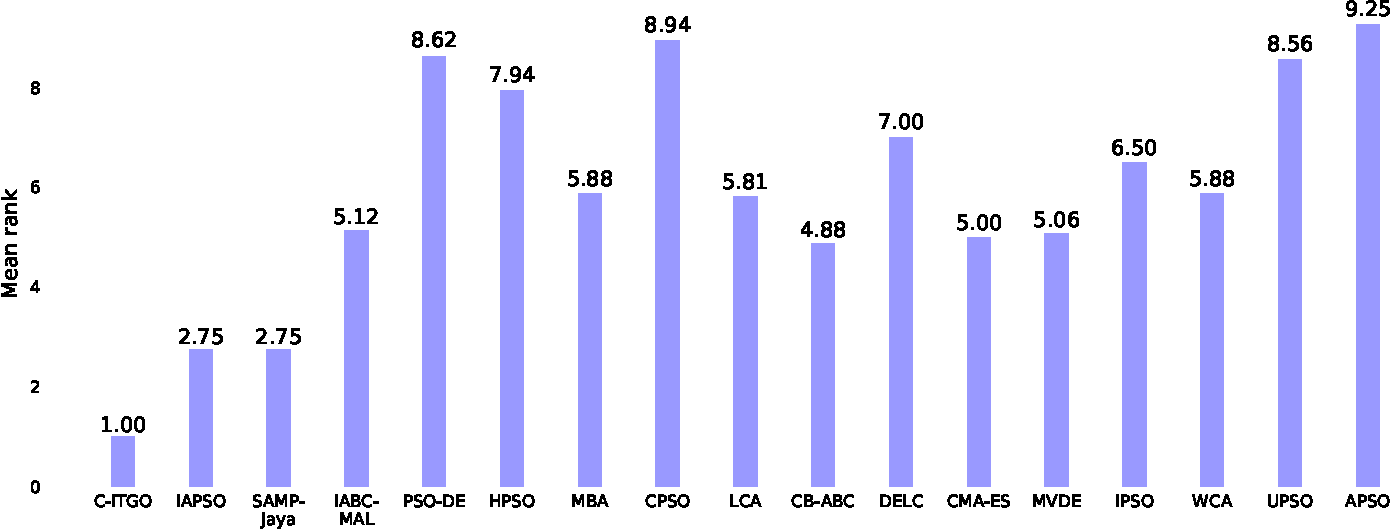
\includegraphics[scale=0.6]{img/Statistics/SkillMack_3-crop.pdf}
    \end{center}
    \captionsetup{justification=centering}
    \vspace*{-4mm}
    \caption{Mean rank plot for all methods that solve at least three problems.}\label{fig:SkillMack_3}
\end{figure}



We also show in Table \ref{tab:SkillMack_5} the results of applying the Skillings-Mack test to the methods that solved at least five problems. For this case, the value of the Skillings-Mack statistic is 44.23462786 with an approximate p-value of 7E-06 calculated from the chi-squared distribution with 11 degrees of freedom. The difference between the results reported in Table \ref{tab:SkillMack_3} is mainly due to the reduction of the number of methods, and the exclusion of some methods that performed well, but in four or fewer problems, such as SAMP-Jaya.

\begin{table}[h]
    \tiny
    \begin{center}
    
    \begin{tabular}{ | P{3.0cm} | P{3.0cm} | }

    \hline

    \rule{0pt}{3ex}
    \textbf{Algorithms} & \textbf{Skillings-Mack ranks}  \\
    \hline

    \rule{0pt}{3ex}
    C-ITGO & 1.0 \\[1em]

    \rule{0pt}{3ex}
    IAPSO & 2.375 \\[1em]

    \rule{0pt}{3ex}
    IABC-MAL & 4.3125 \\[1em]

    \rule{0pt}{3ex}
    PSO-DE & 7.5625 \\[1em]

    \rule{0pt}{3ex}
    MBA & 5.125 \\[1em]

    \rule{0pt}{3ex}
    LCA & 4.875 \\[1em]

    \rule{0pt}{3ex}
    DELC & 5.9375 \\[1em]

    \rule{0pt}{3ex}
    CMA-ES & 4.1875 \\[1em]

    \rule{0pt}{3ex}
    MVDE & 4.25 \\[1em]

    \rule{0pt}{3ex}
    IPSO & 5.4375 \\[1em]

    \rule{0pt}{3ex}
    WCA & 4.9375 \\[1em]

    \rule{0pt}{3ex}
    APSO & 7.75 \\[1em]


    \hline
    
    \rule{0pt}{3ex}    
    \textbf{Skillings-Mack Statistic} & 44.23462786 \\[1em]

    \hline

    \rule{0pt}{3ex}    
    \textbf{p-value} & 7E-06 \\[1em]

    \hline

    \rule{0pt}{3ex}    
    $\bm{\chi^2}$ & 19.67513757 \\[1em]

    \hline

    \end{tabular}
    \end{center}
    \vspace*{-4mm}
    \caption{Skillings-Mack test for methods solving at least five problems. \\[1em]}
    \label{tab:SkillMack_5}
\end{table}

\begin{figure}[bp]
    \begin{center}
    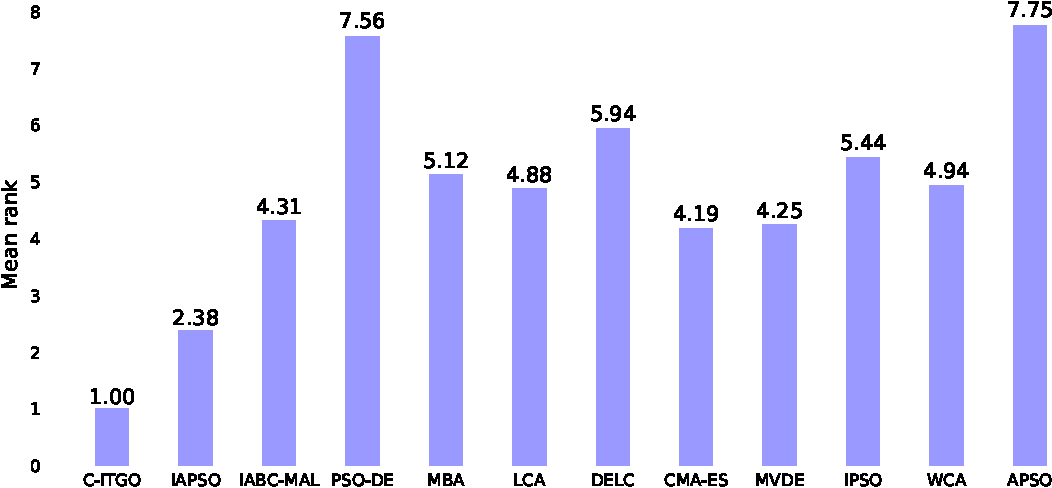
\includegraphics[scale=0.6]{img/Statistics/SkillMack_5-crop.pdf}
    \end{center}
    \captionsetup{justification=centering}
    \vspace*{-4mm}
    \caption{Mean rank plot for all methods that solve at least five problems.}\label{fig:SkillMack_5}
\end{figure}

We see again that C-ITGO has a mean rank of 1.0, far less than IAPSO with 2.375, standing in second place. The plot for the mean rank is shown in Figure \ref{fig:SkillMack_5}. The p-value (7E-06) for this case is also very small, rejecting the null hypothesis at critical level of $\alpha$ = 0.05 or $\alpha$ = 0.01.


We also present in Table \ref{tab:SignedTest} the results of applying the pairwise signed test, comparing C-ITGO against the same methods presented in Table \ref{tab:SkillMack_5} and considering the same performance metric. Here, a "+" represents that C-ITGO outperforms the corresponding method, a "=" represents a tie, and a "-" represents a loss (C-ITGO has worse performance than the corresponding method). If a method does not solve a certain problem, that entry is ignored (marked with "*"). The last row shows the final sum of the number of "+", "=" and "-" for all methods.

\begin{table}[h]
    \tiny
    \begin{center}

    \begin{tabular}{ P{0.7cm} P{0.7cm} P{0.7cm} P{0.8cm} P{0.7cm} P{0.7cm} P{0.7cm} P{0.7cm} P{0.7cm} P{0.7cm} P{0.7cm} P{0.7cm} P{0.7cm}  }
    

    \textbf{Eng. Prob.} & \multicolumn{1}{|c}{C-ITGO} & IAPSO & IABC-MAL & PSO-DE & MBA & LCA & DELC & CMA-ES & MVDE & IPSO & WCA & APSO  \\
    \hline


    \rule{0pt}{5ex}
    WB & \multicolumn{1}{|c}{\textbf{940.68}}     & 12,500 & 15,000 & 66,000 & 47,340 & 15,000 & 20,000 & 4,658 & 15,000 & 20,000 & 46,450 & 50,000 \\
       &                  \multicolumn{1}{|c}{}   &    +   &    +   &    +   &    +   &    +   &    +  &    +   &  +     &    +   &   +    &    +   \\

    \rule{0pt}{7ex}
    TC & \multicolumn{1}{|c}{\textbf{535.08}} & 2,000 & 15,000 & 24,950 & 7,650 & 15,000 & 20,000 & 19,445 & 10,000 & 20,000 & 11,750 & 120,000 \\
       &   \multicolumn{1}{|c}{}              &    +  &    +   &    +  &    +   &    +   &    +   &   +    &    +   &     +  &    +   &    +    \\

    \rule{0pt}{7ex}
    TB & \multicolumn{1}{|c}{\textbf{136.48}} & * & 15,000 & 17,600 & 13,280 & * & 10,000 &  1,706 & 7,000 & * & * & * \\
       &           \multicolumn{1}{|c}{}      &   &    +   &    +   &    +   &   &   +    &   +   &    +   &   &   &  \\

    \rule{0pt}{7ex}
    SRI & \multicolumn{1}{|c}{\textbf{856.40}} & 6,000 & * & * & * & 24,000 & * & * & * & 20,000 & * & 30,000 \\
        &           \multicolumn{1}{|c}{}      &    +  &   &   &   &    +   &   &   &   &    +   &   &    +   \\

    \rule{0pt}{7ex}
    SRII & \multicolumn{1}{|c}{\textbf{491.24}} & 6,000 & 15,000 & 54,350 & 6,300 & 24,000 & 30,000 & 12,998 & 30,000 & 20,000 & 15,150 & 30,000 \\
         &  \multicolumn{1}{|c}{}               &    +  &    +   &   +    &    +  &    +   &    +   &    +   &    +   &   +    &   +    &    +    \\


    \rule{0pt}{7ex}
    PV  & \multicolumn{1}{|c}{\textbf{1101.64}} & 7,500 & 15,000 & 42,100 & 70,650 & 24,000 & 30,000 & 30,018 & 15,000 & 20,000 & 27,500 & 200,000 \\
        &   \multicolumn{1}{|c}{}               &    +  &    +   &   +    &   +    &    +   &   +    &    +   &    +   &    +   &   +    &   +     \\

    \rule{0pt}{7ex}
    GT  & \multicolumn{1}{|c}{\textbf{773.0}} & 800 & * & * & 1,120 & * & * & * & * & * & * & 8,000 \\
        &   \multicolumn{1}{|c}{}             &  +  &   &   &   +  &   &   &   &    &   &   &  +   \\


    \rule{0pt}{7ex}
    MD  & \multicolumn{1}{|c}{\textbf{286.48}} & 400 & * & * & * & * & * & * & * & 20,000 & 500 & 2,000 \\
        &   \multicolumn{1}{|c}{}              &  +  &   &   &  &   &   &   &  &   +    &  +  &  +   \\

    \hline
    
    \rule{0pt}{5ex}
     \textbf{+/=/-} &  \multicolumn{1}{|c}{}  &   \textbf{7/0/0} &   \textbf{5/0/0} &  \textbf{5/0/0} &  \textbf{6/0/0} &  \textbf{5/0/0} &  \textbf{5/0/0} &  \textbf{5/0/0} &  \textbf{5/0/0} &   \textbf{6/0/0} &   \textbf{5/0/0} &   \textbf{7/0/0}  \\
        



    \end{tabular}
    \end{center}
    \captionsetup{justification=centering}
    \caption{The signed test comparing C-ITGO against the other methods that solved at least five problems. Empty entries are represented by *. \\[1em]}
    \label{tab:SignedTest}
\end{table}

As we can see from Table \ref{tab:SignedTest}, C-ITGO always has a better MNFEs than any method for all problems, so there are only "+" entries. Following the guidelines presented in \cite{Friedman}, we can conclude that C-ITGO always achieves a p-value of at least 0.05 when compared to the methods of Table \ref{tab:SignedTest}.


To prove the superior convergence of C-ITGO, we present one more nonparametric statistical test, the Wilcoxon signed rank test, also described in \cite{Friedman}. This is a more robust approach to a pairwise statistical comparison than the previous test, that aims to detect a significant difference between the means of two competing techniques. 

The results shown in Table \ref{tab:Wilcoxon} were generated using the R package \textit{wilcoxon.test}, considering C-ITGO against the other algorithms. Empty entries (problems not solved by some method) are treated by default.
%Methods that solve fewer problems have a higher uncertainty regarding its distribution, consequently having a higher p-value.

\begin{table*}[h]
    \tiny
    \begin{center}
    
    \begin{tabular}{ P{1.0cm} P{1.0cm} P{1.2cm} P{1.0cm} P{1.0cm} P{1.0cm} P{1.0cm} P{1.0cm} }
                     &         &          &          &          &         &           &         \\[2em]
                     &  IAPSO  & IABC-MAL &    MBA   &    LCA   & CMA-ES  &   MVDE    & APSO    \\[1em]
    \cline{2-8}
    \rule{0pt}{3ex}
    \textbf{p-value} & 0.01606 & 0.001661 & 0.001207 & 0.002025 & 0.002155 & 0.002129 & 0.0007229 \\


    \end{tabular}
    \end{center}
    \vspace*{-4mm}
    \captionsetup{justification=centering}
    \caption{Wilcoxon signed rank test comparing C-ITGO against other methods that solved at least five problems. \\[2em]}
    \label{tab:Wilcoxon}
\end{table*}


Given that C-ITGO always had the best MNFEs when compared to all the other methods, as the Table \ref{tab:Wilcoxon} states, C-ITGO shows a improvement over IABC-MAL, MBA, LCA, CMA-ES, MVDE and APSO  with a level of significance $\alpha$ = 0.01, and over IAPSO with a level of significance $\alpha$ = 0.02.